\subsection{CLT -- Examples}
We will draw a random sample of size n from the following distributions:
\begin{itemize}
%\item Standard normal (the \code{rnorm(n,0,1)} function).
%\item Poisson with rate parameter $\lambda=3$ (use \code{rpois(, 3)}).
\item Exponential with rate parameter 5.5 (use \code{rexp(n, 5.5)}).
\item Binomial with probability 0.15.
\end{itemize}

In each case, we will plot a histogram of the sample, and overlay the probability density function on top of it.  We will repeat it 10,000 times and each time calculate the sample mean. Then, we will plot a histogram of the 10,000 sample means.

\subsubsection{Exponential distribution}

\begin{knitrout}
\definecolor{shadecolor}{rgb}{0.969, 0.969, 0.969}\color{fgcolor}\begin{kframe}
\begin{alltt}
\hlcom{# one iteration to show the actual distribution of the sample (not normal)}
\hlstd{n} \hlkwb{<-} \hlnum{100}
\hlstd{samp} \hlkwb{<-} \hlkwd{rexp}\hlstd{(n,} \hlnum{5.5}\hlstd{)}
\hlkwd{hist}\hlstd{(samp,} \hlkwc{freq} \hlstd{= F,} \hlkwc{breaks}\hlstd{=}\hlnum{20}\hlstd{,}\hlkwc{main}\hlstd{=}\hlstr{""}\hlstd{,} \hlkwc{xlab}\hlstd{=}\hlstr{"x"}\hlstd{,} \hlkwc{border}\hlstd{=}\hlstr{"white"}\hlstd{)} \hlcom{# show the empirical distribution}
\hlstd{xs} \hlkwb{<-} \hlkwd{seq}\hlstd{(}\hlnum{0}\hlstd{,} \hlkwd{max}\hlstd{(samp),} \hlkwc{length}\hlstd{=}\hlnum{1000}\hlstd{)}
\hlkwd{lines}\hlstd{(xs,} \hlkwd{dexp}\hlstd{(xs,}\hlnum{5.5}\hlstd{),} \hlkwc{lwd}\hlstd{=}\hlnum{3}\hlstd{,} \hlkwc{col}\hlstd{=}\hlnum{2}\hlstd{)} \hlcom{# show the true distribution}
\end{alltt}
\end{kframe}\begin{figure}

{\centering 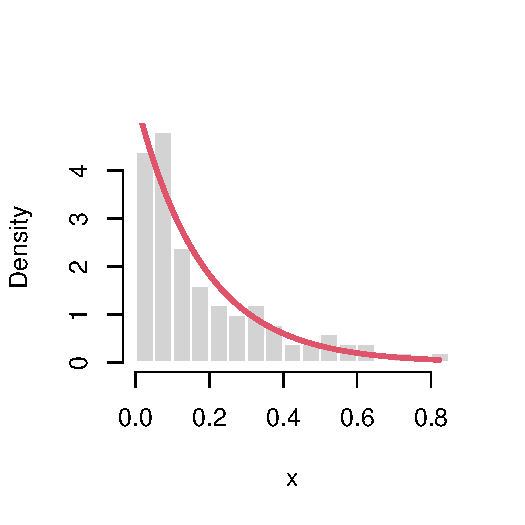
\includegraphics[width=\maxwidth]{figure/intro-lln5-0-1} 

}

\caption[Simulated data from an exponential distribution]{Simulated data from an exponential distribution.}\label{fig:intro-lln5-0}
\end{figure}

\end{knitrout}

Notice that the distribution is very skewed, and not at all like a normal distribution.
To understand the CLT, we will compare the distribution of the 10,000 means for two different sample sizes, 50 and 500.

\begin{knitrout}
\definecolor{shadecolor}{rgb}{0.969, 0.969, 0.969}\color{fgcolor}\begin{kframe}
\begin{alltt}
\hlcom{# 10000 iterations - show the distribution of the sample means:}
\hlstd{n} \hlkwb{<-} \hlnum{50}
\hlstd{allMeans} \hlkwb{<-} \hlkwd{rep}\hlstd{(}\hlnum{0}\hlstd{,} \hlnum{10000}\hlstd{)}
\hlkwa{for} \hlstd{(i} \hlkwa{in} \hlnum{1}\hlopt{:}\hlnum{10000}\hlstd{) \{}
  \hlstd{samp} \hlkwb{<-} \hlkwd{rexp}\hlstd{(n,}\hlnum{5.5}\hlstd{)}
  \hlstd{allMeans[i]} \hlkwb{<-} \hlkwd{mean}\hlstd{(samp)}
\hlstd{\}}
\hlkwd{par}\hlstd{(}\hlkwc{mfrow}\hlstd{=}\hlkwd{c}\hlstd{(}\hlnum{1}\hlstd{,}\hlnum{2}\hlstd{))}
\hlstd{m} \hlkwb{<-} \hlkwd{min}\hlstd{(allMeans)}
\hlstd{M} \hlkwb{<-} \hlkwd{max}\hlstd{(allMeans)}
\hlkwd{hist}\hlstd{(allMeans,} \hlkwc{freq} \hlstd{= F,} \hlkwc{breaks}\hlstd{=}\hlnum{40}\hlstd{,} \hlkwc{xlim}\hlstd{=}\hlkwd{c}\hlstd{(m, M),} \hlkwc{main}\hlstd{=}\hlstr{""}\hlstd{,} \hlkwc{xlab}\hlstd{=}\hlstr{"Sample mean"}\hlstd{,} \hlkwc{border}\hlstd{=}\hlstr{"white"}\hlstd{,} \hlkwc{col}\hlstd{=}\hlstr{"orchid"}\hlstd{)}
\hlkwd{abline}\hlstd{(}\hlkwc{v}\hlstd{=}\hlnum{1}\hlopt{/}\hlnum{5.5}\hlstd{,} \hlkwc{lwd}\hlstd{=}\hlnum{3}\hlstd{,} \hlkwc{col}\hlstd{=}\hlstr{"green"}\hlstd{)}

\hlcom{# repeat, this time with a larger sample size:}
\hlcom{# 10000 iterations - show the distribution of the sample means:}
\hlstd{n} \hlkwb{<-} \hlnum{500}
\hlstd{allMeans} \hlkwb{<-} \hlkwd{rep}\hlstd{(}\hlnum{0}\hlstd{,} \hlnum{10000}\hlstd{)}
\hlkwa{for} \hlstd{(i} \hlkwa{in} \hlnum{1}\hlopt{:}\hlnum{10000}\hlstd{) \{}
  \hlstd{samp} \hlkwb{<-} \hlkwd{rexp}\hlstd{(n,}\hlnum{5.5}\hlstd{)}
  \hlstd{allMeans[i]} \hlkwb{<-} \hlkwd{mean}\hlstd{(samp)}
\hlstd{\}}
\hlkwd{hist}\hlstd{(allMeans,} \hlkwc{freq} \hlstd{= F,} \hlkwc{breaks}\hlstd{=}\hlnum{40}\hlstd{,} \hlkwc{xlim}\hlstd{=}\hlkwd{c}\hlstd{(m, M),} \hlkwc{main}\hlstd{=}\hlstr{""}\hlstd{,} \hlkwc{xlab}\hlstd{=}\hlstr{"Sample mean"}\hlstd{,} \hlkwc{border}\hlstd{=}\hlstr{"white"}\hlstd{,} \hlkwc{col}\hlstd{=}\hlstr{"orange"}\hlstd{)}
\hlkwd{abline}\hlstd{(}\hlkwc{v}\hlstd{=}\hlnum{1}\hlopt{/}\hlnum{5.5}\hlstd{,} \hlkwc{lwd}\hlstd{=}\hlnum{3}\hlstd{,} \hlkwc{col}\hlstd{=}\hlstr{"green"}\hlstd{)}
\end{alltt}
\end{kframe}\begin{figure}

{\centering 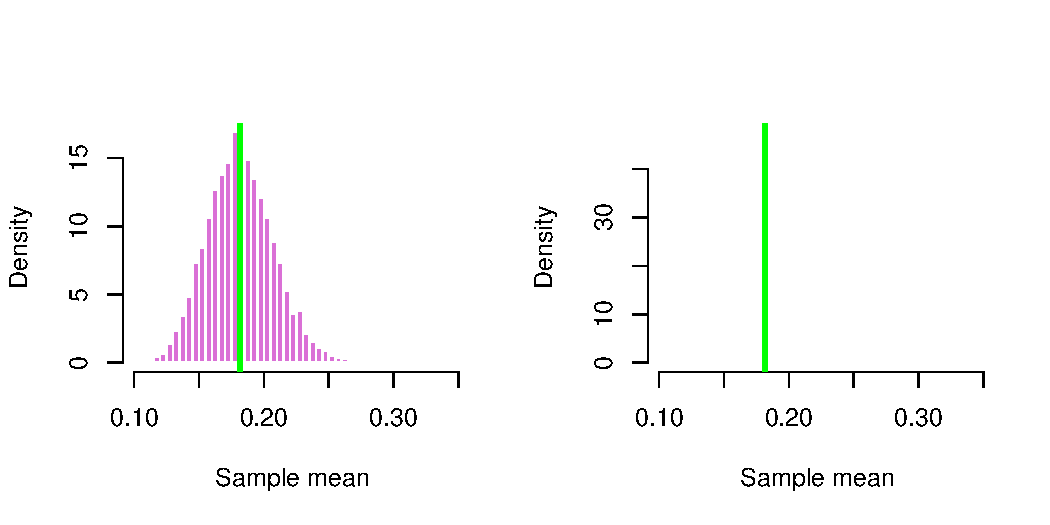
\includegraphics[width=\maxwidth]{figure/intro-lln5-1-1} 

}

\caption[The distribution of the sample mean from 10,000 simulated data from an exponential distribution]{The distribution of the sample mean from 10,000 simulated data from an exponential distribution. Left: $n=50$, right: $n=500$}\label{fig:intro-lln5-1}
\end{figure}

\begin{kframe}\begin{alltt}
\hlkwd{par}\hlstd{(}\hlkwc{mfrow}\hlstd{=}\hlkwd{c}\hlstd{(}\hlnum{1}\hlstd{,}\hlnum{1}\hlstd{))}
\end{alltt}
\end{kframe}
\end{knitrout}

The mean is estimated quite accurately in both cases, and the overall shape of the 10,000 sample means has the shape of a normal distribution. However, the spread (variance) of the distribution decreases as the sample size increases.

\subsubsection{Binomial distribution}
In this example, our data come from a discrete and skewed distribution.

\begin{knitrout}
\definecolor{shadecolor}{rgb}{0.969, 0.969, 0.969}\color{fgcolor}\begin{kframe}
\begin{alltt}
\hlcom{# 10000 iterations - show the distribution of the sample means:}
\hlstd{n} \hlkwb{<-} \hlnum{50}
\hlstd{allMeans} \hlkwb{<-} \hlkwd{rep}\hlstd{(}\hlnum{0}\hlstd{,} \hlnum{10000}\hlstd{)}
\hlkwa{for} \hlstd{(i} \hlkwa{in} \hlnum{1}\hlopt{:}\hlnum{10000}\hlstd{) \{}
  \hlstd{samp} \hlkwb{<-} \hlkwd{rbinom}\hlstd{(n,}\hlnum{1}\hlstd{,}\hlnum{0.15}\hlstd{)}
  \hlstd{allMeans[i]} \hlkwb{<-} \hlkwd{mean}\hlstd{(samp)}
\hlstd{\}}
\hlkwd{par}\hlstd{(}\hlkwc{mfrow}\hlstd{=}\hlkwd{c}\hlstd{(}\hlnum{1}\hlstd{,}\hlnum{2}\hlstd{))}
\hlstd{m} \hlkwb{<-} \hlkwd{min}\hlstd{(allMeans)}
\hlstd{M} \hlkwb{<-} \hlkwd{max}\hlstd{(allMeans)}
\hlkwd{hist}\hlstd{(allMeans,} \hlkwc{freq} \hlstd{= F,} \hlkwc{breaks}\hlstd{=}\hlnum{40}\hlstd{,} \hlkwc{xlim}\hlstd{=}\hlkwd{c}\hlstd{(m, M),} \hlkwc{main}\hlstd{=}\hlstr{""}\hlstd{,} \hlkwc{xlab}\hlstd{=}\hlstr{"Sample mean"}\hlstd{,} \hlkwc{border}\hlstd{=}\hlstr{"white"}\hlstd{,} \hlkwc{col}\hlstd{=}\hlstr{"orchid"}\hlstd{)}
\hlkwd{abline}\hlstd{(}\hlkwc{v}\hlstd{=}\hlnum{0.15}\hlstd{,} \hlkwc{lwd}\hlstd{=}\hlnum{3}\hlstd{,} \hlkwc{col}\hlstd{=}\hlstr{"green"}\hlstd{)}

\hlcom{# repeat, this time with a larger sample size:}
\hlcom{# 10000 iterations - show the distribution of the sample means:}
\hlstd{n} \hlkwb{<-} \hlnum{500}
\hlstd{allMeans} \hlkwb{<-} \hlkwd{rep}\hlstd{(}\hlnum{0}\hlstd{,} \hlnum{10000}\hlstd{)}
\hlkwa{for} \hlstd{(i} \hlkwa{in} \hlnum{1}\hlopt{:}\hlnum{10000}\hlstd{) \{}
  \hlstd{samp} \hlkwb{<-} \hlkwd{rbinom}\hlstd{(n,}\hlnum{1}\hlstd{,}\hlnum{0.15}\hlstd{)}
  \hlstd{allMeans[i]} \hlkwb{<-} \hlkwd{mean}\hlstd{(samp)}
\hlstd{\}}
\hlkwd{hist}\hlstd{(allMeans,} \hlkwc{freq} \hlstd{= F,} \hlkwc{breaks}\hlstd{=}\hlnum{40}\hlstd{,} \hlkwc{xlim}\hlstd{=}\hlkwd{c}\hlstd{(m, M),} \hlkwc{main}\hlstd{=}\hlstr{""}\hlstd{,} \hlkwc{xlab}\hlstd{=}\hlstr{"Sample mean"}\hlstd{,} \hlkwc{border}\hlstd{=}\hlstr{"white"}\hlstd{,} \hlkwc{col}\hlstd{=}\hlstr{"orange"}\hlstd{)}
\hlkwd{abline}\hlstd{(}\hlkwc{v}\hlstd{=}\hlnum{0.15}\hlstd{,} \hlkwc{lwd}\hlstd{=}\hlnum{3}\hlstd{,} \hlkwc{col}\hlstd{=}\hlstr{"green"}\hlstd{)}
\end{alltt}
\end{kframe}\begin{figure}

{\centering 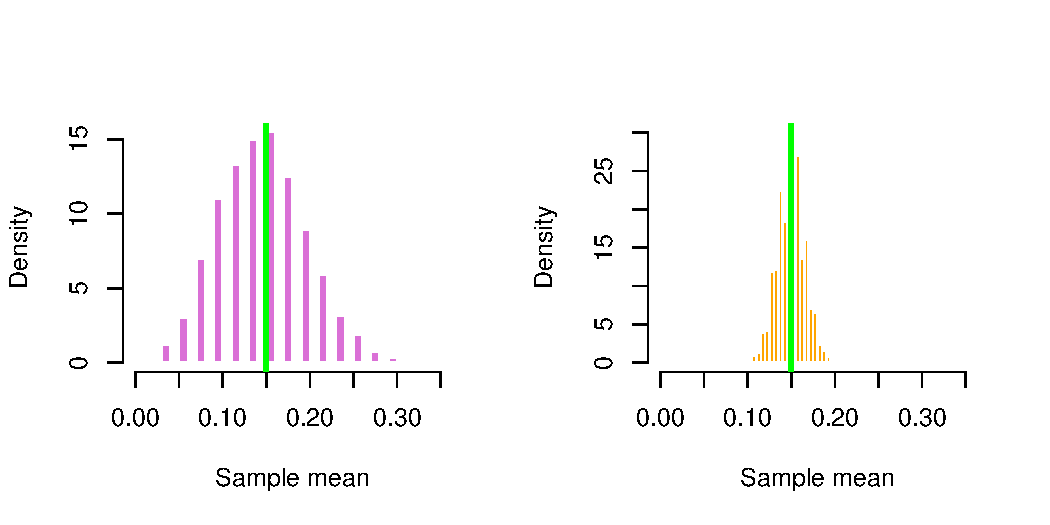
\includegraphics[width=\maxwidth]{figure/intro-lln5-2-1} 

}

\caption[The distribution of the sample mean from 10,000 simulated data from a binomial distribution]{The distribution of the sample mean from 10,000 simulated data from a binomial distribution. Left: $n=50$, right: $n=500$}\label{fig:intro-lln5-2}
\end{figure}

\begin{kframe}\begin{alltt}
\hlkwd{par}\hlstd{(}\hlkwc{mfrow}\hlstd{=}\hlkwd{c}\hlstd{(}\hlnum{1}\hlstd{,}\hlnum{1}\hlstd{))}
\end{alltt}
\end{kframe}
\end{knitrout}

Notice that because p=0.15 is quite small, when n=50 the shape of the distribution of sample means is still a bit skewed, but when n is large the bell shape appears! 

\subsubsection{Application to child births -- boy/girl ratio}
In 2021 the boy to girl birth ratio in the USA is estimated to be 1.05. If we took a random sample of 300 newborns across the USA, how many do you expect to be boys?

\begin{knitrout}
\definecolor{shadecolor}{rgb}{0.969, 0.969, 0.969}\color{fgcolor}\begin{kframe}
\begin{alltt}
\hlstd{b2g} \hlkwb{<-} \hlnum{1.05} \hlcom{# B/G}
\hlcom{# We need B/(B+G)}
\hlcom{# Since B/G=1.05, B=1.05G, so:}
\hlstd{pboy} \hlkwb{<-} \hlnum{1.05}\hlopt{/}\hlstd{(}\hlnum{1}\hlopt{+}\hlnum{1.05}\hlstd{)}
\hlstd{n} \hlkwb{<-} \hlnum{300}
\hlstd{nsim} \hlkwb{<-} \hlnum{1}
\hlkwd{set.seed}\hlstd{(}\hlnum{100091}\hlstd{)}
\hlstd{boysInSample} \hlkwb{<-} \hlkwd{rbinom}\hlstd{(nsim, n, pboy)}
\hlkwd{cat}\hlstd{(}\hlstr{"Prob. boy:"}\hlstd{, pboy,} \hlstr{". Simulated number of boys in a sample of 300 is:"}\hlstd{,} \hlkwd{mean}\hlstd{(boysInSample),}\hlstr{"\textbackslash{}n"}\hlstd{)}
\end{alltt}
\begin{verbatim}
## Prob. boy: 0.5121951 . Simulated number of boys in a sample of 300 is: 151
\end{verbatim}
\end{kframe}
\end{knitrout}

Would it be very surprising if we actually see 148 in the random sample?\\
Suppose we took a sample of 3,000, instead. Would is be surprising if we observed 1,480 boys?\\
How about if we took a sample of 30,000, instead. Would is be surprising if we observed 14,800 boys?

The probability of a boy birth does not depend on the sample size, and we calculated it to be 0.512, so the expected number of boys when the sample size is 300, 3000, and 30000 is 151, 1510, and 15100, respectively. So, it may appear that actually observing 148 instead of 151 is as likely as observing 1480 instead of 1510, or 14800 instead of 15100, but that is not true!
The CLT tells us that when the sample size increases, the dispersion of the sample means around the true mean gets smaller and smaller. This is demonstrated in the code below. The green vertical line represents the expected number of boys, and the red one represents the observed ones. Notice that as we increase the sample size, the likelihood of the observed number of boys (148, 1480, 14800) gets smaller. When $n=30000$ the red line is well outside the range of the simulated sample means.

\begin{knitrout}
\definecolor{shadecolor}{rgb}{0.969, 0.969, 0.969}\color{fgcolor}\begin{kframe}
\begin{alltt}
\hlstd{n} \hlkwb{<-} \hlnum{300}
\hlstd{nsim} \hlkwb{<-} \hlnum{10000}
\hlkwd{par}\hlstd{(}\hlkwc{mfrow}\hlstd{=}\hlkwd{c}\hlstd{(}\hlnum{1}\hlstd{,}\hlnum{3}\hlstd{))}
\hlkwd{set.seed}\hlstd{(}\hlnum{100091}\hlstd{)}
\hlstd{boysInSample} \hlkwb{<-} \hlkwd{rbinom}\hlstd{(nsim, n, pboy)}
\hlkwd{hist}\hlstd{(boysInSample,} \hlkwc{breaks}\hlstd{=}\hlnum{30}\hlstd{,}\hlkwc{border}\hlstd{=}\hlstr{"white"}\hlstd{,} \hlkwc{xlim}\hlstd{=}\hlkwd{c}\hlstd{(}\hlnum{130}\hlstd{,}\hlnum{190}\hlstd{),} \hlkwc{freq}\hlstd{=}\hlnum{FALSE}\hlstd{,} \hlkwc{main}\hlstd{=}\hlstr{"n=300"}\hlstd{)}
\hlkwd{abline}\hlstd{(}\hlkwc{v}\hlstd{=pboy}\hlopt{*}\hlstd{n,} \hlkwc{col}\hlstd{=}\hlnum{3}\hlstd{,} \hlkwc{lwd}\hlstd{=}\hlnum{3}\hlstd{)}
\hlkwd{abline}\hlstd{(}\hlkwc{v}\hlstd{=}\hlnum{148}\hlstd{,} \hlkwc{col}\hlstd{=}\hlnum{2}\hlstd{,} \hlkwc{lwd}\hlstd{=}\hlnum{2}\hlstd{)}

\hlcom{# sample size is 10 times larger:}
\hlstd{boysInSample2} \hlkwb{<-} \hlkwd{rbinom}\hlstd{(nsim,} \hlnum{10}\hlopt{*}\hlstd{n, pboy)}
\hlkwd{hist}\hlstd{(boysInSample2,} \hlkwc{breaks}\hlstd{=}\hlnum{30}\hlstd{,} \hlkwc{border}\hlstd{=}\hlstr{"white"}\hlstd{,} \hlkwc{xlim}\hlstd{=}\hlkwd{c}\hlstd{(}\hlnum{1400}\hlstd{,}\hlnum{1700}\hlstd{),} \hlkwc{freq}\hlstd{=}\hlnum{FALSE}\hlstd{,} \hlkwc{main}\hlstd{=}\hlstr{"n=3,000"}\hlstd{)}
\hlkwd{abline}\hlstd{(}\hlkwc{v}\hlstd{=pboy}\hlopt{*}\hlnum{10}\hlopt{*}\hlstd{n,} \hlkwc{col}\hlstd{=}\hlnum{3}\hlstd{,} \hlkwc{lwd}\hlstd{=}\hlnum{3}\hlstd{)}
\hlkwd{abline}\hlstd{(}\hlkwc{v}\hlstd{=}\hlnum{1480}\hlstd{,} \hlkwc{col}\hlstd{=}\hlnum{2}\hlstd{,} \hlkwc{lwd}\hlstd{=}\hlnum{2}\hlstd{)}

\hlcom{# sample size is 100 times larger than the original example:}
\hlstd{boysInSample3} \hlkwb{<-} \hlkwd{rbinom}\hlstd{(nsim,} \hlnum{100}\hlopt{*}\hlstd{n, pboy)}
\hlkwd{hist}\hlstd{(boysInSample3,} \hlkwc{breaks}\hlstd{=}\hlnum{30}\hlstd{,}\hlkwc{border}\hlstd{=}\hlstr{"white"}\hlstd{,} \hlkwc{xlim}\hlstd{=}\hlkwd{c}\hlstd{(}\hlnum{14500}\hlstd{,}\hlnum{16000}\hlstd{),} \hlkwc{freq}\hlstd{=}\hlnum{FALSE}\hlstd{,} \hlkwc{main}\hlstd{=}\hlstr{"n=30,000"}\hlstd{)}
\hlkwd{abline}\hlstd{(}\hlkwc{v}\hlstd{=pboy}\hlopt{*}\hlnum{100}\hlopt{*}\hlstd{n,} \hlkwc{col}\hlstd{=}\hlnum{3}\hlstd{,} \hlkwc{lwd}\hlstd{=}\hlnum{3}\hlstd{)}
\hlkwd{abline}\hlstd{(}\hlkwc{v}\hlstd{=}\hlnum{14800}\hlstd{,} \hlkwc{col}\hlstd{=}\hlnum{2}\hlstd{,} \hlkwc{lwd}\hlstd{=}\hlnum{2}\hlstd{)}
\end{alltt}
\end{kframe}\begin{figure}

{\centering 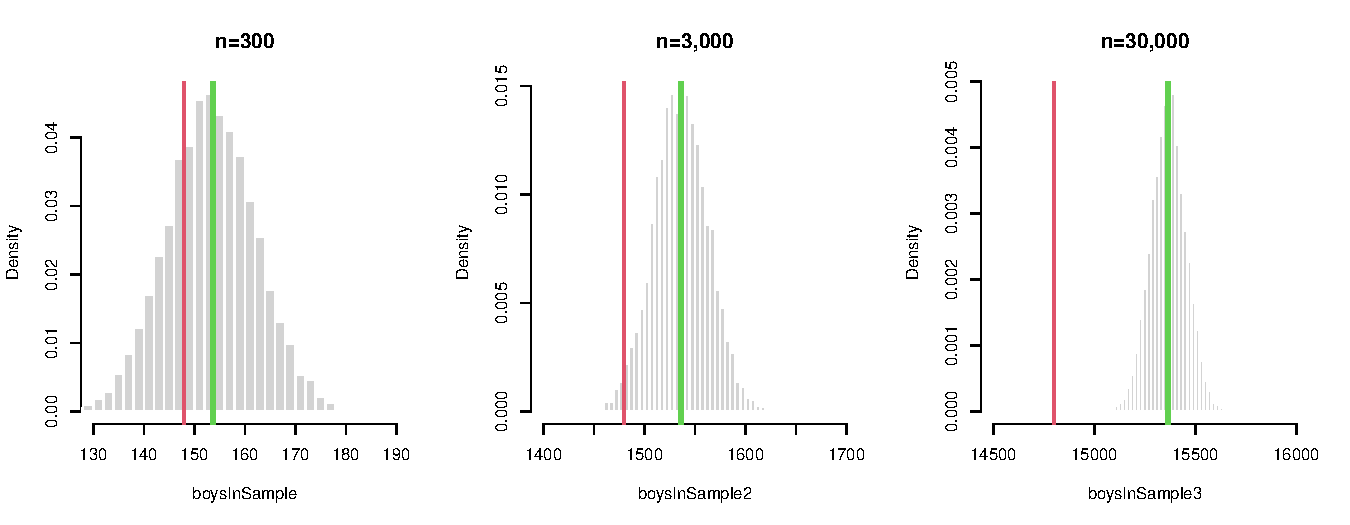
\includegraphics[width=\maxwidth]{figure/intro-lln5-4-1} 

}

\caption[Number of boy births]{Number of boy births.}\label{fig:intro-lln5-4}
\end{figure}

\begin{kframe}\begin{alltt}
\hlkwd{par}\hlstd{(}\hlkwc{mfrow}\hlstd{=}\hlkwd{c}\hlstd{(}\hlnum{1}\hlstd{,}\hlnum{1}\hlstd{))}
\end{alltt}
\end{kframe}
\end{knitrout}

\subsection{Summary}
The LLN and CLT are very powerful results. Keep in mind that in real-life when we do not know the true distribution, we can usually get just \textit{one sample}, not 10,000 like we did in our simulations.
However, these theorems tell us that as long as this one sample is large enough, we can get a very good approximation for the distribution of the sample mean, if we \textit{could} get multiple samples.
Not only that, but regardless of the distribution of the data, the sample mean will have a normal distribution with mean which is equal to the true mean of the original distribution (even if it's skewed, or discrete), and the variance of the sample mean will shrink as we increase the sample size. This is very convenient for testing hypotheses and constructing confidence intervals (next chapter).

To conclude, let us revisit the IQ example, where we assumed that in the general population IQ scores have a normal distribution with mean=100 and  standard deviation =15.
We drew a sample of 200 people, and calculated the sample mean and standard deviation, which turned out to be 99.4, and 15.6, respectively.
The red curve shows the true density function, and the dashed green one shows the one estimated from the sample of 200 people. They are very close.

\begin{knitrout}
\definecolor{shadecolor}{rgb}{0.969, 0.969, 0.969}\color{fgcolor}\begin{kframe}
\begin{alltt}
\hlkwd{set.seed}\hlstd{(}\hlnum{95473}\hlstd{)}
\hlstd{n} \hlkwb{<-} \hlnum{200}
\hlstd{samp} \hlkwb{<-} \hlkwd{rnorm}\hlstd{(n,} \hlnum{100}\hlstd{,} \hlnum{15}\hlstd{)}
\hlkwd{hist}\hlstd{(samp,} \hlkwc{freq}\hlstd{=}\hlnum{FALSE}\hlstd{,} \hlkwc{main}\hlstd{=}\hlstr{""}\hlstd{,} \hlkwc{xlab}\hlstd{=}\hlstr{"IQ score"}\hlstd{,} \hlkwc{border}\hlstd{=}\hlstr{"white"}\hlstd{,} \hlkwc{col}\hlstd{=}\hlstr{"lightblue"}\hlstd{)}
\hlstd{xs} \hlkwb{<-} \hlkwd{seq}\hlstd{(}\hlnum{40}\hlstd{,}\hlnum{180}\hlstd{,} \hlkwc{length}\hlstd{=}\hlnum{1000}\hlstd{)}
\hlkwd{lines}\hlstd{(xs,} \hlkwd{dnorm}\hlstd{(xs,} \hlnum{100}\hlstd{,} \hlnum{15}\hlstd{),} \hlkwc{col}\hlstd{=}\hlnum{2}\hlstd{,} \hlkwc{lwd}\hlstd{=}\hlnum{3}\hlstd{)}
\hlkwd{lines}\hlstd{(xs,} \hlkwd{dnorm}\hlstd{(xs,} \hlkwd{mean}\hlstd{(samp),} \hlkwd{sd}\hlstd{(samp)),} \hlkwc{col}\hlstd{=}\hlnum{3}\hlstd{,} \hlkwc{lwd}\hlstd{=}\hlnum{3}\hlstd{,} \hlkwc{lty}\hlstd{=}\hlnum{2}\hlstd{)}
\end{alltt}
\end{kframe}\begin{figure}

{\centering 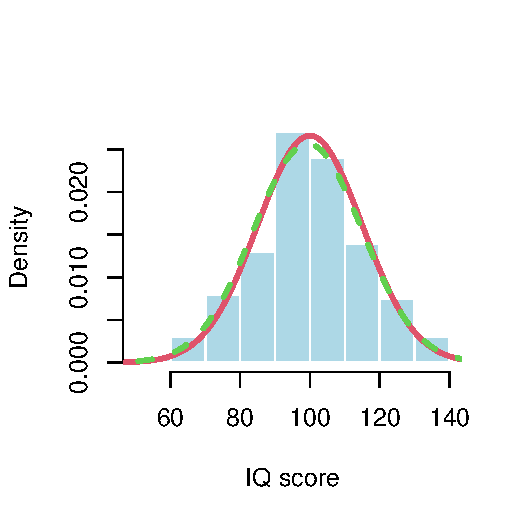
\includegraphics[width=\maxwidth]{figure/intro-lln5-5-1} 

}

\caption[Simulated IQ scores]{Simulated IQ scores.}\label{fig:intro-lln5-5}
\end{figure}

\end{knitrout}

To answer the question how likely  it is to find a person with IQ greater than 150, we can calculate the area of the right tail of the distribution:

\begin{knitrout}
\definecolor{shadecolor}{rgb}{0.969, 0.969, 0.969}\color{fgcolor}\begin{kframe}
\begin{alltt}
\hlkwd{cat}\hlstd{(}\hlnum{1}\hlopt{-}\hlkwd{pnorm}\hlstd{(}\hlnum{150}\hlstd{,} \hlkwc{mean}\hlstd{=}\hlkwd{mean}\hlstd{(samp),} \hlkwc{sd}\hlstd{=}\hlkwd{sd}\hlstd{(samp)),}\hlstr{"\textbackslash{}n"}\hlstd{)}
\end{alltt}
\begin{verbatim}
## 0.0005699322
\end{verbatim}
\end{kframe}
\end{knitrout}
A very select group, indeed.

In order to be accepted to the Mensa club a person has to be in the top 2\% of the IQ distribution. In order to find the minimum score required in order to be a Mensa member, we use the \code{quantile} function, if we want to use the data, or the \code{qnorm} function to get the threshold from distribution of the entire population:

\begin{knitrout}
\definecolor{shadecolor}{rgb}{0.969, 0.969, 0.969}\color{fgcolor}\begin{kframe}
\begin{alltt}
\hlstd{mensacutoff} \hlkwb{<-} \hlkwd{round}\hlstd{(}\hlkwd{quantile}\hlstd{(samp,}\hlkwc{probs} \hlstd{=} \hlnum{0.98}\hlstd{))}
\hlkwd{cat}\hlstd{(}\hlstr{"Sample quantile:"}\hlstd{, mensacutoff,}\hlstr{"\textbackslash{}n"}\hlstd{)}
\end{alltt}
\begin{verbatim}
## Sample quantile: 131
\end{verbatim}
\begin{alltt}
\hlkwd{cat}\hlstd{(}\hlstr{"Population quantile:"}\hlstd{,} \hlkwd{qnorm}\hlstd{(}\hlnum{0.98}\hlstd{,} \hlkwc{mean}\hlstd{=}\hlkwd{mean}\hlstd{(samp),} \hlkwc{sd}\hlstd{=}\hlkwd{sd}\hlstd{(samp)),}\hlstr{"\textbackslash{}n"}\hlstd{)}
\end{alltt}
\begin{verbatim}
## Population quantile: 131.3356
\end{verbatim}
\end{kframe}
\end{knitrout}

We can show it graphically:
\begin{knitrout}
\definecolor{shadecolor}{rgb}{0.969, 0.969, 0.969}\color{fgcolor}\begin{kframe}
\begin{alltt}
\hlstd{xs} \hlkwb{<-} \hlkwd{seq}\hlstd{(}\hlnum{40}\hlstd{,}\hlnum{180}\hlstd{,} \hlkwc{length}\hlstd{=}\hlnum{1000}\hlstd{)}
\hlkwd{plot}\hlstd{(xs,} \hlkwd{dnorm}\hlstd{(xs,} \hlnum{100}\hlstd{,} \hlnum{15}\hlstd{),} \hlkwc{col}\hlstd{=}\hlnum{2}\hlstd{,} \hlkwc{lwd}\hlstd{=}\hlnum{2}\hlstd{,} \hlkwc{type}\hlstd{=}\hlstr{'l'}\hlstd{,} \hlkwc{axes}\hlstd{=F,} \hlkwc{ylab}\hlstd{=}\hlstr{""}\hlstd{,} \hlkwc{xlab}\hlstd{=}\hlstr{"IQ"}\hlstd{)}
\hlkwd{axis}\hlstd{(}\hlnum{1}\hlstd{);} \hlkwd{axis}\hlstd{(}\hlnum{2}\hlstd{)}
\hlstd{xx} \hlkwb{<-} \hlkwd{seq}\hlstd{(}\hlkwd{qnorm}\hlstd{(}\hlnum{0.98}\hlstd{,} \hlkwc{mean}\hlstd{=}\hlkwd{mean}\hlstd{(samp),} \hlkwc{sd}\hlstd{=}\hlkwd{sd}\hlstd{(samp)),} \hlnum{200}\hlstd{,} \hlkwc{length}\hlstd{=}\hlnum{20}\hlstd{)}
\hlstd{yy} \hlkwb{<-} \hlkwd{dnorm}\hlstd{(xx,} \hlnum{100}\hlstd{,} \hlnum{15}\hlstd{)}
\hlkwd{polygon}\hlstd{(}\hlkwd{c}\hlstd{(xx,} \hlkwd{rev}\hlstd{(xx)),} \hlkwd{c}\hlstd{(}\hlkwd{rep}\hlstd{(}\hlnum{0}\hlstd{,}\hlkwd{length}\hlstd{(xx)),} \hlkwd{rev}\hlstd{(yy)),} \hlkwc{col}\hlstd{=}\hlstr{"green"}\hlstd{,} \hlkwc{border}\hlstd{=}\hlstr{"green"}\hlstd{,} \hlkwc{lwd}\hlstd{=}\hlnum{2}\hlstd{)}
\end{alltt}
\end{kframe}\begin{figure}

{\centering 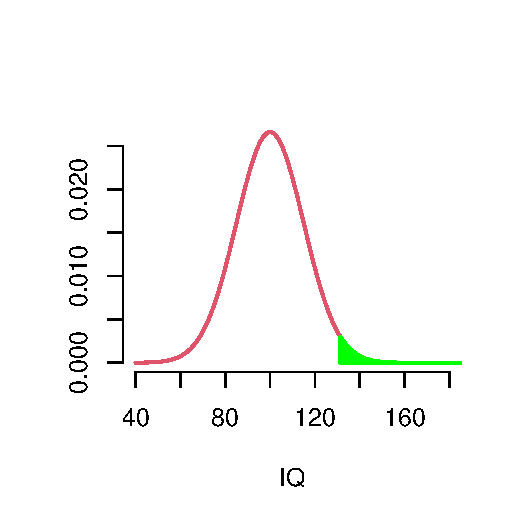
\includegraphics[width=\maxwidth]{figure/intro-lln5-8-1} 

}

\caption[The distribution of IQ's and the acceptance range to the Mensa club]{The distribution of IQ's and the acceptance range to the Mensa club.}\label{fig:intro-lln5-8}
\end{figure}

\end{knitrout}

In chapter \ref{ch:hypothesis} we will see how the CLT can be use to form hypotheses and construct confident intervals. For example, we will be able to answer questions such as: "You are given the IQ test results of 13 people and they are: 139, 104, 115, 151, 116, 141, 117, 105, 134, 155, 130, 139, 121.
Is this group different than the overall population?"

